
\section{Inference}
\label{section:inference}
The GAIA-2 model supports a range of inference tasks that showcase its flexibility and controllability across video generation scenarios. These tasks are unified by a shared denoising process operating in the latent space, followed by decoding into pixel space via the video tokenizer.


\begin{figure}[t]
    \centering
    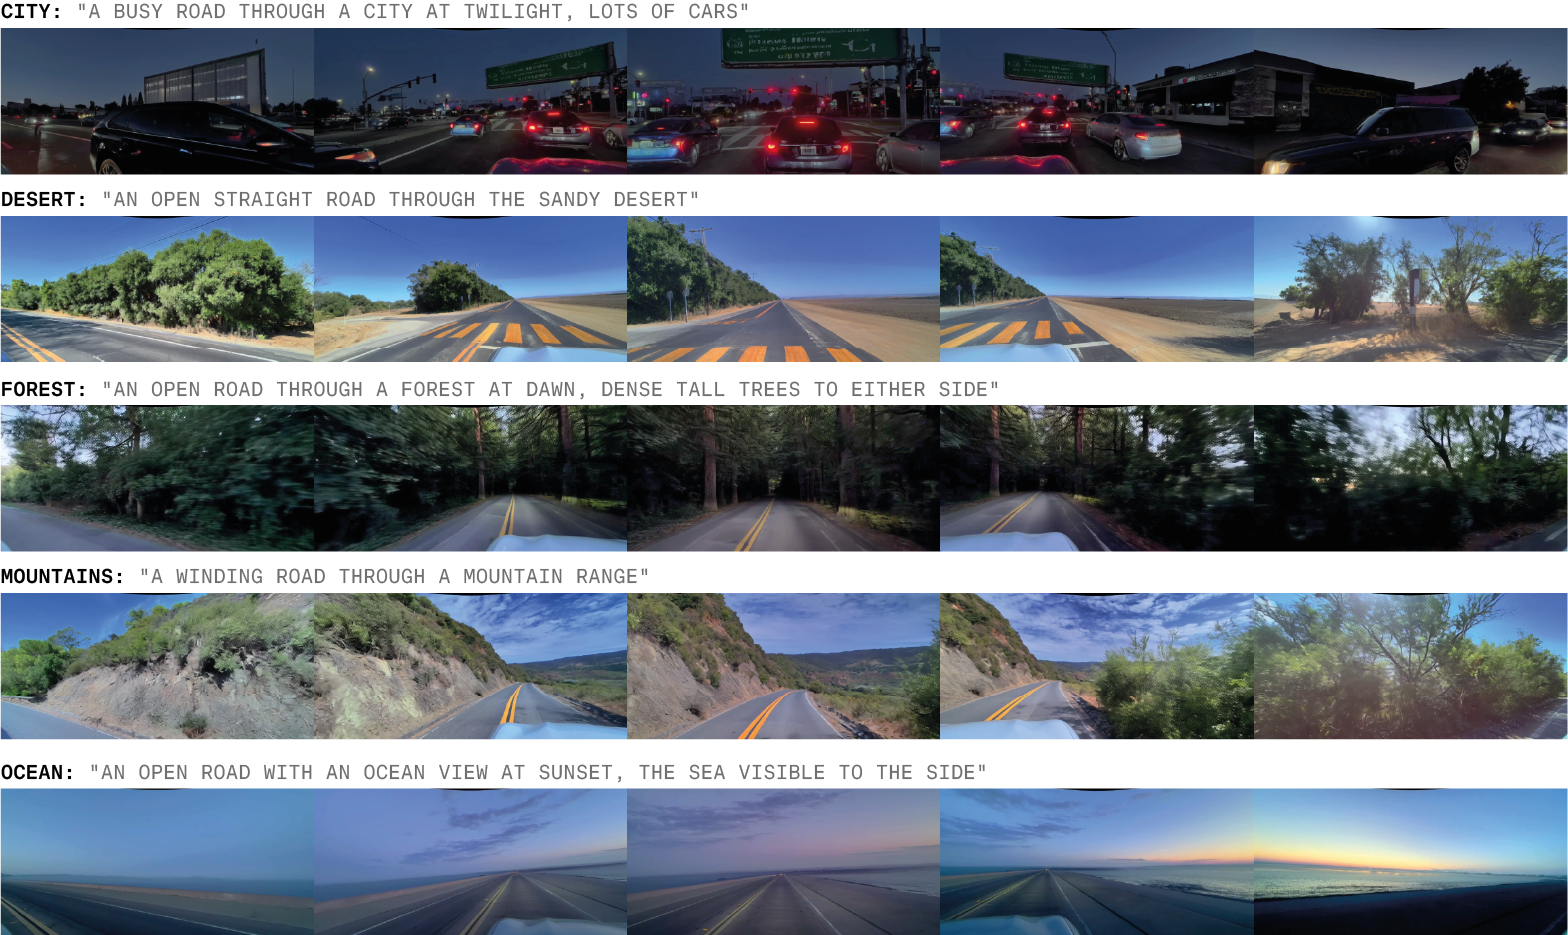
\includegraphics[width=1.0\textwidth]{Figures/clip.png}
    \caption{\textbf{CLIP conditioning.} Conditioning GAIA-2 generations with text prompts encoded through the CLIP text encoder provides nuanced control over environmental features.}
    \label{fig:clip}
\end{figure}


\paragraph{Inference Tasks.}
We consider four primary inference modes, each illustrating a distinct capability of the model:

\begin{itemize} 
\item \textbf{Generation from scratch} involves sampling pure Gaussian noise and denoising them with guidance from conditioning variables defined in Section~\ref{subsubsection:conditioning}. The resulting latents are then decoded to video frames using the video tokenizer decoder, with temporally consistent outputs produced via the rolling window decoding mechanism illustrated in Figure~\ref{fig:video-tokenizer}.

\item \textbf{Autoregressive prediction} enables forecasting future latents from a sequence of past context latents. Given an initial context window of $k=3$ temporal latents, the model predicts the next set of latents, appends it to the context, and repeats the process using a sliding window. This approach allows for long-horizon rollouts while incorporating conditioning signals such as ego motion. An example is provided in Figure~\ref{fig:unsafe-actions}.

\item \textbf{Inpainting} allows selective modification of video content. A spatial-temporal mask is applied to the latent input, and the masked regions are regenerated via conditional denoising. Optional guidance from dynamic agent conditioning (e.g., agent locations) can steer the generation within the masked area. An example is shown in~\Cref{fig:inpainting}.

\item \textbf{Scene editing} is achieved by partially noising latents extracted from real video, followed by denoising with altered conditioning. This enables targeted semantic or stylistic transformations—such as changing the weather, time of day, or road layout—without re-generating the full scene. \Cref{fig:noisedenoise} illustrates this capability.
\end{itemize}
These modes demonstrate that GAIA-2 can serve as a general-purpose simulator for a wide variety of scene manipulation tasks, whether starting from noise, context, or existing video.


\paragraph{Inference Noise Schedule.}
For all inference tasks, we adopt the linear-quadratic noise schedule introduced by \cite{polyak2024movie}. This schedule begins with linearly spaced noise levels, which are effective for capturing coarse scene layouts and motion patterns. In later stages, the schedule transitions to quadratically spaced steps that allow more efficient refinement of high-frequency visual details. This hybrid approach improves both generation quality and computational efficiency. In our experiments, we use a fixed number of 50 denoising steps.



\paragraph{Classifier-Free Guidance.}
Classifier-free guidance (CFG) is not used by default during inference. However, for challenging or out-of-distribution scenarios, such as those involving rare edge cases or unusual agent configurations (e.g., Figure~\ref{fig:cuboids}), we activate CFG with a guidance scale ranging from 2 to 20, depending on the complexity of the scene.

In scenarios involving dynamic agent conditioning, where the latent tokens associated with agent-specific regions are known a priori, we apply spatially selective CFG. In this case, guidance is applied only to the spatial locations influenced by the conditioning (e.g., 3D bounding boxes), which enhances generation quality in targeted regions without unnecessarily affecting the rest of the scene. This targeted approach enables more precise control over scene elements while preserving global coherence.
